\documentclass[12pt, a4paper]{article}

\newcommand*{\Author}{Roberto Gesteira Miñarro}
\newcommand*{\Keywords}{Neural network, decision tree, clustering, association rules}
\newcommand*{\Subject}{Phishing detection}
\newcommand*{\Title}{Phishing detection}

\usepackage{amsmath}
\usepackage{amssymb}
\usepackage[english]{babel}
\usepackage[font=small, labelfont=bf, labelsep=period]{caption}
\usepackage{csquotes}
\usepackage{datetime}
\usepackage{float}
\usepackage[T1]{fontenc}
\usepackage[bmargin=3cm, lmargin=3cm, rmargin=3cm, tmargin=3cm]{geometry}
\usepackage{graphicx}
\usepackage[breaklinks]{hyperref}
\usepackage[utf8]{inputenc}
\usepackage[newfloat]{minted}
\usepackage{parskip}
\usepackage{siunitx}
\usepackage{titletoc}
\usepackage{xcolor}

\renewcommand{\textit}{\textsl}

\colorlet{bgcolor}{gray!10}

\newcommand{\itab}[1]{\hspace{0em}\rlap{#1}}
\newcommand{\tab}[1]{\hspace{.14\textwidth}\rlap{#1}}

\titlecontents{figure}[0em]{}{\itab{\textbf{\figurename~\thecontentslabel.}} \tab{\ }}{}{\titlerule*[0.8pc]{.}\contentspage\vspace{8pt}}[]

\providecommand{\sectionname}{Section}

\addto\captionsenglish{\renewcommand{\contentsname}{Table of contents\newline}}
\addto\captionsenglish{\renewcommand{\figurename}{Figure}}
\addto\captionsenglish{\renewcommand{\listfigurename}{List of figures\newline}}

\newcommand*{\figref}[1]{\figurename~\ref{fig:#1}}

\hypersetup{
  colorlinks=true,
  linkcolor=black,
  pdfauthor=\Author,
  pdfkeywords=\Keywords,
  pdfsubject=\Subject,
  pdftitle=\Title,
  urlcolor=blue
}
\urlstyle{same}

\graphicspath{{./images/}}

\newcommand{\figcaption}[4][H]{
  \begin{figure}[#1]
    \centering
    \includegraphics[width=#4\textwidth]{#2}
    \caption{#3}
    \label{fig:#2}
  \end{figure}
}

\newcommand*{\sourcedir}{../src}

\usemintedstyle{vs}

\newcommand*{\codebgnocaption}[3][fontsize=\scriptsize, linenos=false]{
  \begin{listing}[H]
    \inputminted[bgcolor=bgcolor, #1]{#3}{\sourcedir/#2}
  \end{listing}
  \vspace{-1.2cm}
}

\newcommand*{\kmeans}{$K$-means}
\newcommand*{\ML}{Machine Learning}

\title{\underline{\textbf{Phishing detection}}}
\author{\Author}
\newdate{date}{27}{05}{2021}
\date{\displaydate{date}}

\begin{document}

  \vspace{3cm}
  \maketitle

  \newpage
  \tableofcontents

  \newpage
  \listoffigures

  \newpage
  \section*{Introduction}
    \addcontentsline{toc}{section}{Introduction}

    In this project, a dataset analysis based on URL features accessible by HTTP or HTTPS is done, using known \ML\ algorithms.

    The dataset used for the study can be found at \url{https://www.kaggle.com/manishkc06/web-page-phishing-detection}, although the original contents are at \url{https://data.mendeley.com/datasets/c2gw7fy2j4/2}, plus some Python codes to extract the features of provided URL.

    The objective of the analysis is to construct several models that can be used to predict whether an URL contains some kind of phishing depending on the characteristics of that URL. The models development and analysis is done in R.

    As an additional solution, it is intended to develop a tool that can detect if an URL is legitimate or contains phishing. To achieve this, firstly the URL is characterized with a Python script (based on the ones coming with the dataset); and secondly, the obtained features are entered to the models created with R, in order to predict the type of URL.

    As a result, it will be possible to prevent phishing attacks by integrating this tool to browsers and email clients, to analyze an URL and warn users of a potential danger.

  \section{Characterization and exploration of the dataset}

    Firstly, it is necessary to observe the dataset to know the variables that are involved and the number of examples available.

    The original dataset contains $89$ variables and $11\,481$ observations. By experience, it is known that it will be difficult to work with this dataset (above all using clustering algorithms). Therefore, a reduction of the dataset is needed.

    Among the $89$ variables, there are $6$ that always have the same value for all observations. It is obvious that such variables do not give any relevant information and must be deleted from the dataset.

    On the other hand, there exists a variable that can be used as index (i.e. the URL), and the target variable \texttt{status}, which indicates if an URL is legitimate or contains phising.

    To determine if among thhe $81$ variables remaining there is one more important than the others, a principal component analysis (PCA) is done, obtaining the following scree plot:

    \figcaption{pca1.png}{Principal component analysis over the original dataset}{1}

    It can be seen in \figref{pca1.png} that it is not possible to distinguish clearly any important component, because the tallest bar is slightly above \SI{10}{\percent}. Then, another method should be implemented to reduce the size of the dataset.

    There are some binary variables in the dataset that have the same value for more than \SI{90}{\percent} of the examples, which means that these variables do not give useful information. They only highlight a few examples. Hence, this counted examples are deleted, and then the whole variable is deleted (because it will have the same value for all observations).

    The pervious process is repeated until the dataset stabilizes at $47$ variables (considering \texttt{url} and \texttt{status}) and $5\,445$ observations. Now, the dataset is much lighter and is better to work with.

    Anyway, another PCA is done over the reduced dataset in order to check if there exists an important component. Taking a look at \figref{pca2.png}, it is concluded that there are no principal components.

    For the rest of the sections, the reduced dataset is the one that is used.

    \figcaption{pca2.png}{Principal component analysis over the reduced dataset}{1}

    \subsection{Variables in the dataset}

      Once the dataset is defined, it is convenient to know the meanings of each variable. Some of the then are listed below:

      \begin{itemize}
        \item \texttt{url}: Contains the value of the URL, as text.
        \item \texttt{status}: Indicates whether the URL is legitimate or contains phishing.
        \item \texttt{length\_url}: Number of characters of the URL.
        \item \texttt{nb\_dots}: Number of dots (characters) in the URL.
        \item \texttt{https\_token}: `0' if the URL contains \texttt{https} and `1' otherwise.
        \item \texttt{shortening\_service}: `1' if the URL contains the name of a known URL shortener and `0' otherwise.
        \item \texttt{nb\_hyperlinks}: Number of links within the HTML source code of the web page.
        \item \texttt{empty\_title}: `0' if the web page contains a title in the HTML source code (\texttt{<title>John Doe</title>}) and `1' otherwise.
        \item \texttt{google\_index}: `0' if the URL appears in the first page of a Google search and `1' otherwise.
        \item \texttt{page\_rank}: Quality of the web page in a range from 0 to 10.
      \end{itemize}

  \section{Association rules}

    In this section the variables of the dataset are related in order to obtain rules for obtaining interesting dependencies between variables.

    \figref{rules.png} shows the resulting association rules. For example, webpages without title (\texttt{empty\_title=1}) are not shown in Google (\texttt{google\_index=1}); as well as URL that come from a shortener (\texttt{shortening\_service=1}).

    Other interesting rules indicate that an URL contains phishing if the webpage does not have a title (\texttt{empty\_title=1} or if the URL is shortened (\texttt{shortening\_service=1}). Furthermore, if the domain name of the URL is inside a set of known brands (\texttt{domain\_in\_brand=1}), then the URL will be accessible by HTTPS (\texttt{https\_token=0}).

    \figcaption{rules.png}{Resulting association rules}{1}

    The \textit{apriori} algorithm from the \texttt{arules} packet of R has been used to generate these association rules. The rules represented in the graph shwon in \figref{rules.png} have a confidence greater than \SI{50}{\percent}, a coverage less than the unit and they are composed by two elements (there are non rules that involve more than two elements).

    As the \textit{apriori} algorithm requires categorical variables, only the binary variables of the dataset have been used, transformed to factor type. Despite missing information, the resulting rules have a logical explanation and therefore they are relevant.

  \section{Clustering}

    In this section several clustering analyzes are carried out: firstly, hierarchical clustering over the variables of the dataset and then over the observations; and secondly, \kmeans\ over the observations. It is worth mentioning that these algorithms are unsupervised, that is, the models do not know the expected results.

    \subsection{Hierarchical clustering over the variables}

      First, a hierarchical clustering analysis is performed on the variables to verify their similarity. Having normalized the dataset, the \figref{dist_var.png} is obtained, which represents by colors the distances between variables according to the Euclidean metric:

      \figcaption{dist_var.png}{Distances between the variables of the dataset}{1}

      It can be seen that there are two clearly differentiable groups: one containing variables whose distance is smaller and the other containing variables whose distance is grater. These groups are shown in the following dendrogram, obtained from an agglomerative hierarchical clustering (using the \texttt{agnes} packet of R and the Ward's method):

      \figcaption{dend_var.png}{Dendrogram of the variables}{1}

      There are continuous and discrete variables with several possible values within the blue group (such as \texttt{avg\_word\_path} or \texttt{nb\_dots}), whereas the orange group contains mainly binary variables (for instance, \texttt{https\_token} or \texttt{google\_index}).

      This analysis helps to understand the meaning of the variables and to observe similarities among them. A divisive clustering was also performed, but it did not produce a dendrogram as clear as the one in \figref{dend_var.png}.

    \subsection{Hierarchical clustering over the observations}

      At this point, the examples of the dataset are analyzed with hierarchical clustering. Firstly, the best agglomerative method to build the model is computed. As shown below, the best agglomerative coefficient is obtained with Ward's method:

      \begin{minted}[bgcolor=bgcolor]{text}
  average      single    complete        ward
0.9163371   0.8693480   0.9429070   0.9957265
      \end{minted}

      This method results in the dendrogram shown in \figref{ward.png}. It seems that is reasonable to select $3$ groups, which are marked with colors in the figure itself.

      \figcaption{ward.png}{Dendrogram obtained with agglomerative clustering and Ward's method}{1}

      Next, this model is compared to one built with divisive clustering. The result of the divisive one is the following dendrogram:

      \figcaption{diana.png}{Dendrogram obtained with divisive clustering}{1}

      \newpage

      In this case it is more difficult to distinguish groups, although choosing $3$ groups seems to be an acceptable decision, as shown in \figref{diana.png}.

      It is worth mentioning that there is no need for the result to match the URL class, as these models are unsupervised. In fact, both models seem to split the dataset in $3$ groups, not $2$.

      Knowing beforehand that there are two types of URL in the dataset, the models could be tested using confusion matrices and forcing the algorithms to choose $2$ groups. The results obtained when introducing the same dataset the model was trained with, are reflected in the following confusion matrices for the agglomerative and divisive methods, respectively:

      \begin{minted}[bgcolor=bgcolor]{text}
             Reference
Prediction   legitimate   phishing
legitimate         2060       1319
phishing           1337        729

             Reference
Prediction   legitimate   phishing
legitimate         2954        425
phishing            888       1178
      \end{minted}

      As these results are not good (\SI{51.22}{\percent} and \SI{75.89}{\percent} precision), it follows that these algorithms are not useful for the objective of analysis. Moreover, these models are very time-consuming in their training process (they last more than half an hour).

      Like it was said before, clustering algorithms simply make groups according to similarities within observations, which will not always match the class of each observation.

    \subsection{\kmeans}

      Another clustering algorithm is \kmeans, which needs beforehand the number of clusters to group the dataset.

      First, the elbow method is used in order to see the evolution of the WSS depending on the number of clusters $K$, as shown in \figref{elbow.png}.

      This graph does not show a clear value for the number of clusters. Hence, the silhouette method is performed to choose $K$. It can be seen in \figref{silhouette.png} that the most suitable value of $K$ is $2$.

      \figcaption{elbow.png}{Number of clusters according to the elbow method}{1}

      \figcaption{silhouette.png}{Number of clusters according to the silhouette method}{1}

      \newpage

      Once chosen $K$, the model is trained with \kmeans. Despite being an unsupervised model, a training set and a testing set have been used, taking advantage of the fact that the number of clusters equals the number of classes of URL within the dataset.

      The following confusion matrices show the obtained results:

      \begin{minted}[bgcolor=bgcolor]{text}
Train:
             Reference
Prediction   legitimate   phishing
legitimate         1970        581
phishing            608        925

Test:
             Reference
Prediction   legitimate   phishing
legitimate          633        195
phishing            201        332
      \end{minted}

      Again, it follows that \kmeans\ is not an adequate method to analyze the dataset, due to the resulting precisions are \SI{70.89}{\percent} and \SI{70.9}{\percent} en training and testing, respectively. In addition, as a clustering algorithm, there is no need for the result to match the class of the URL.

  \section{Kohonen maps}

    The next analysis is based on Kohonen self-organizing maps. This model is a kind of neural network that can be supervised or unsupervised.

    The main parameters of this model are the number of neurons, the dimensions and the topology of the map. Having performed several tests with different dimensions and topologies, it was observed that a good model was obtained with a hexagonal topology and $3 \times 3$ dimensions ($9$ neurons). The learning coefficient $\alpha$ was configured as the default one of the \texttt{kohonen} packet.

    \subsection{Unsupervised model}

      In \figref{maps.png} it is shown the importance of each variable inside the neurons of the map. Consequently, the reduncancy of some variables can de determined. For instance, variables \texttt{longest\_words\_raw}, \texttt{longest\_word\_path}, \texttt{avg\_words\_raw} and \texttt{avg\_word\_raw} are pretty similar to variable \texttt{length\_url}, due to the fact that their maps have the same colors.

      To continue, these redundant variables are deleted and the model is trained again. The new importance of the variables is shown in \figref{maps_nr.png}.

      \begin{figure}[H]
        \centering
        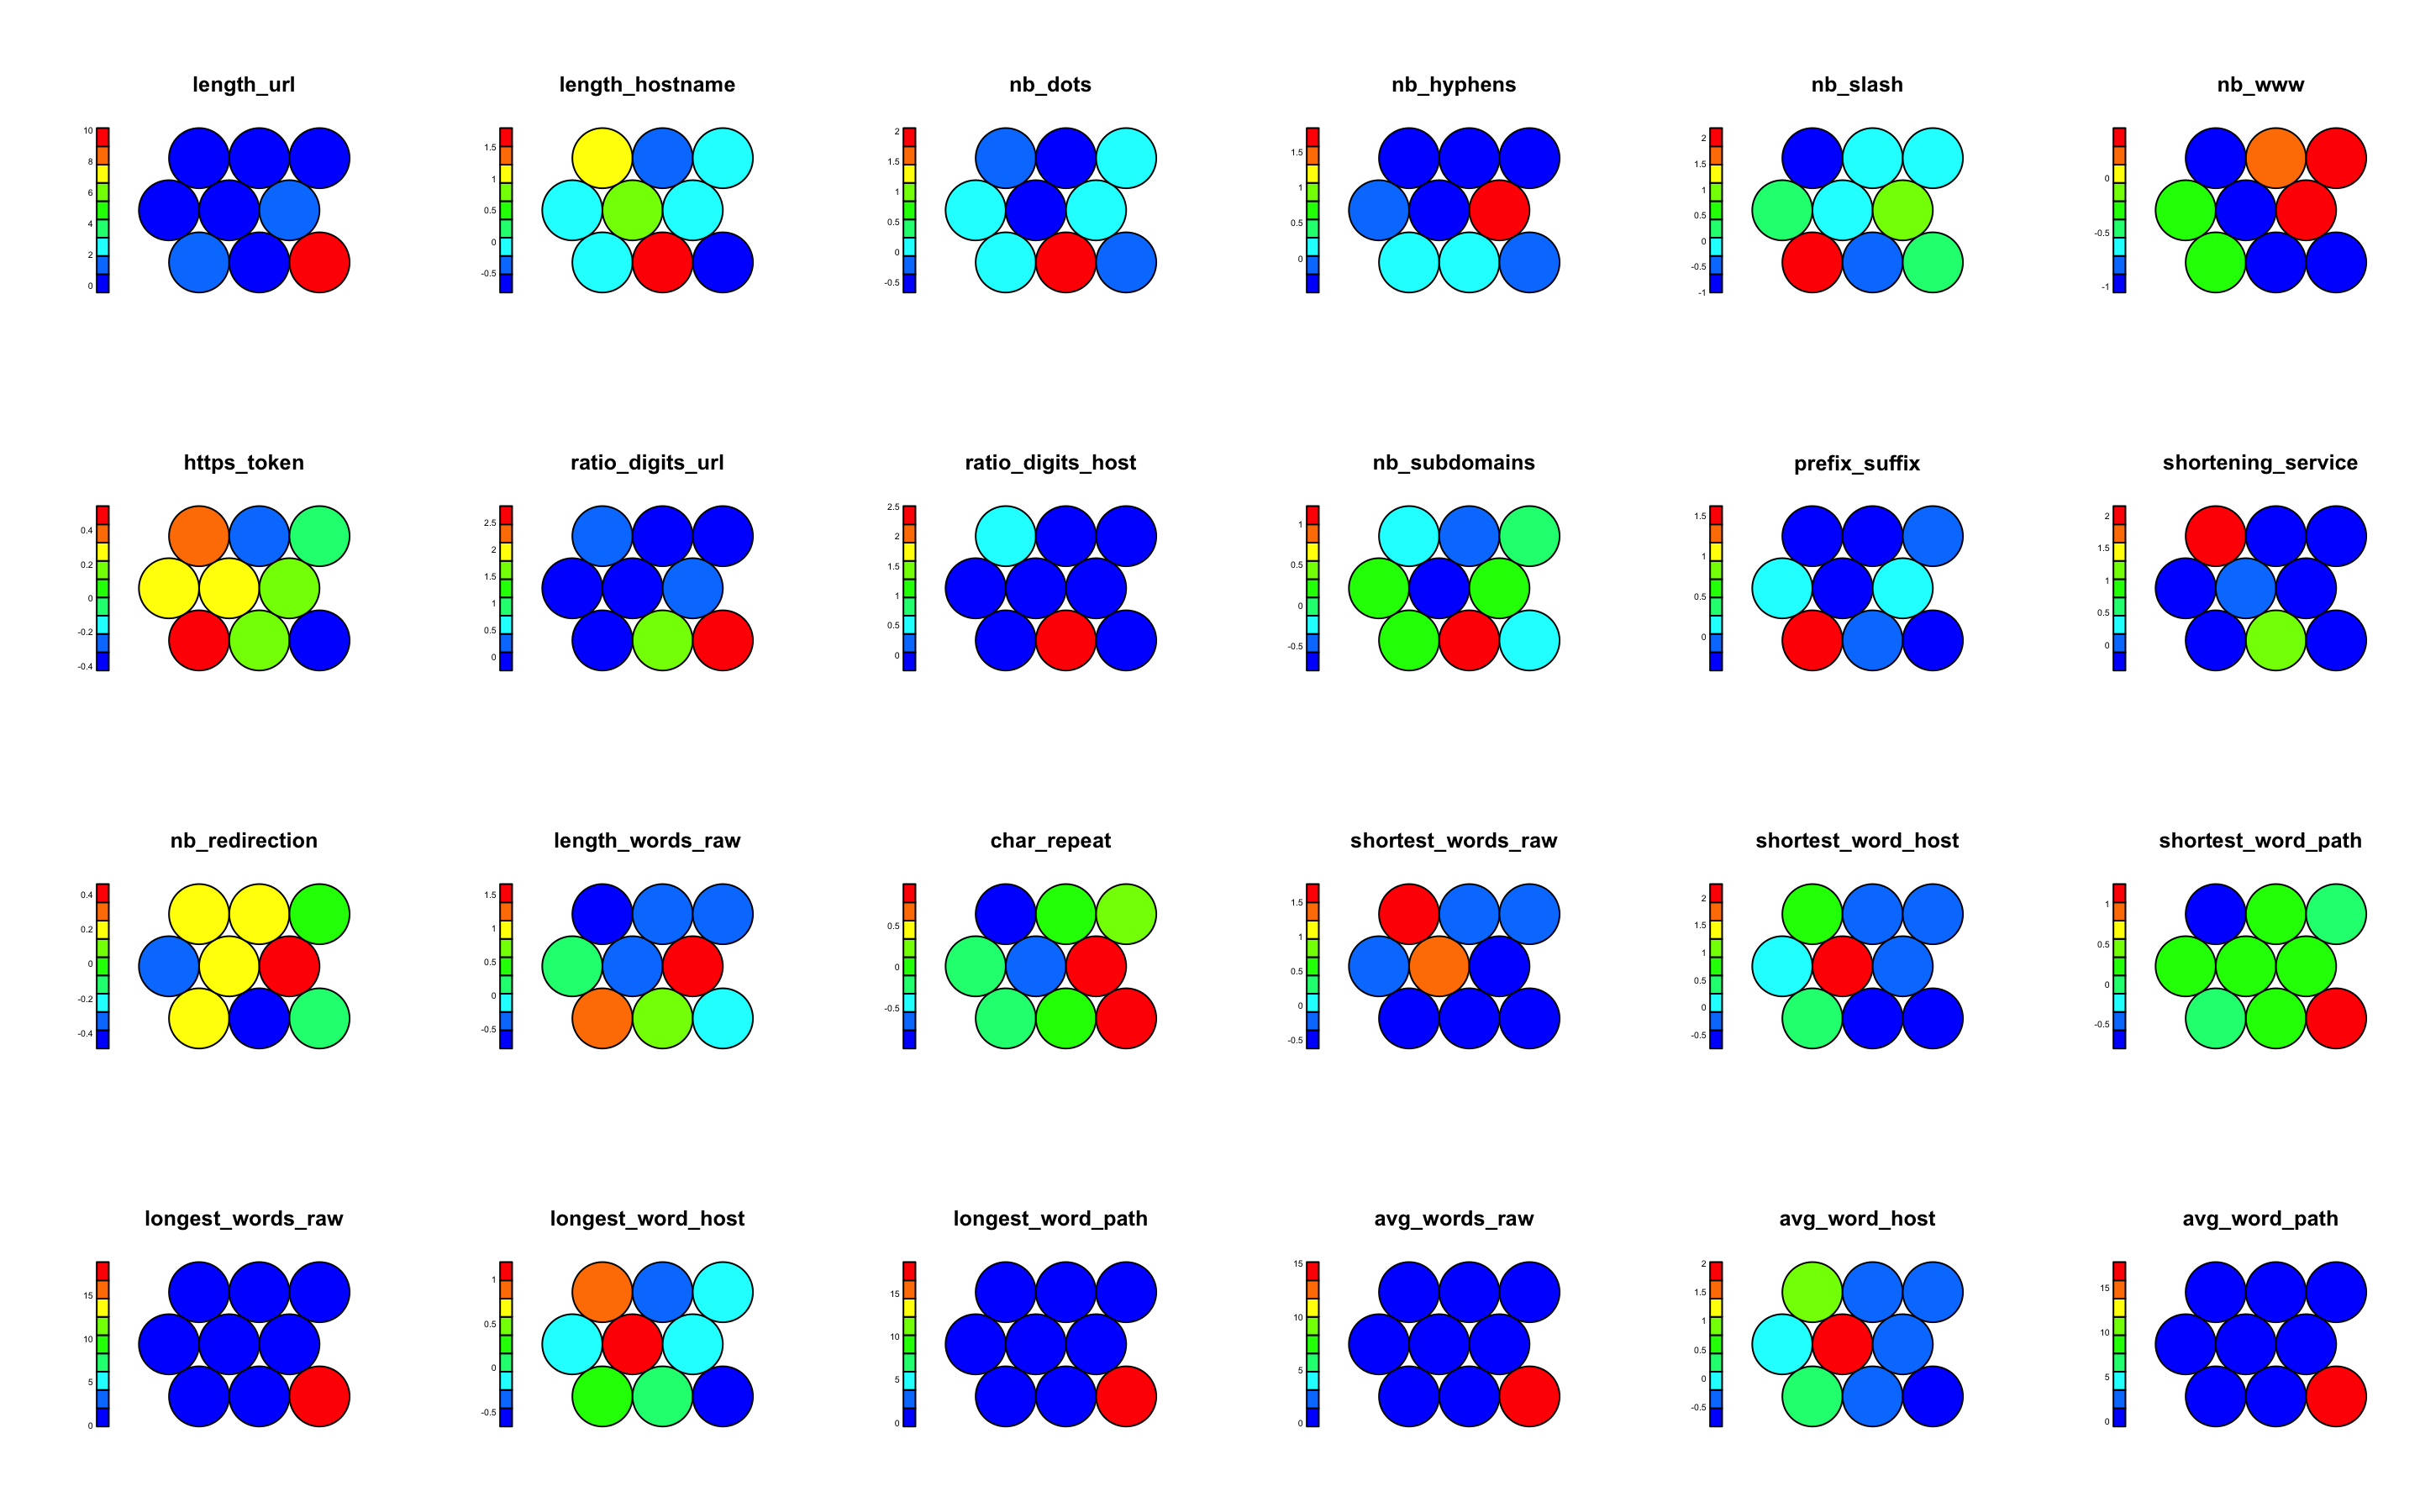
\includegraphics[width=1\textwidth]{maps1.png}
        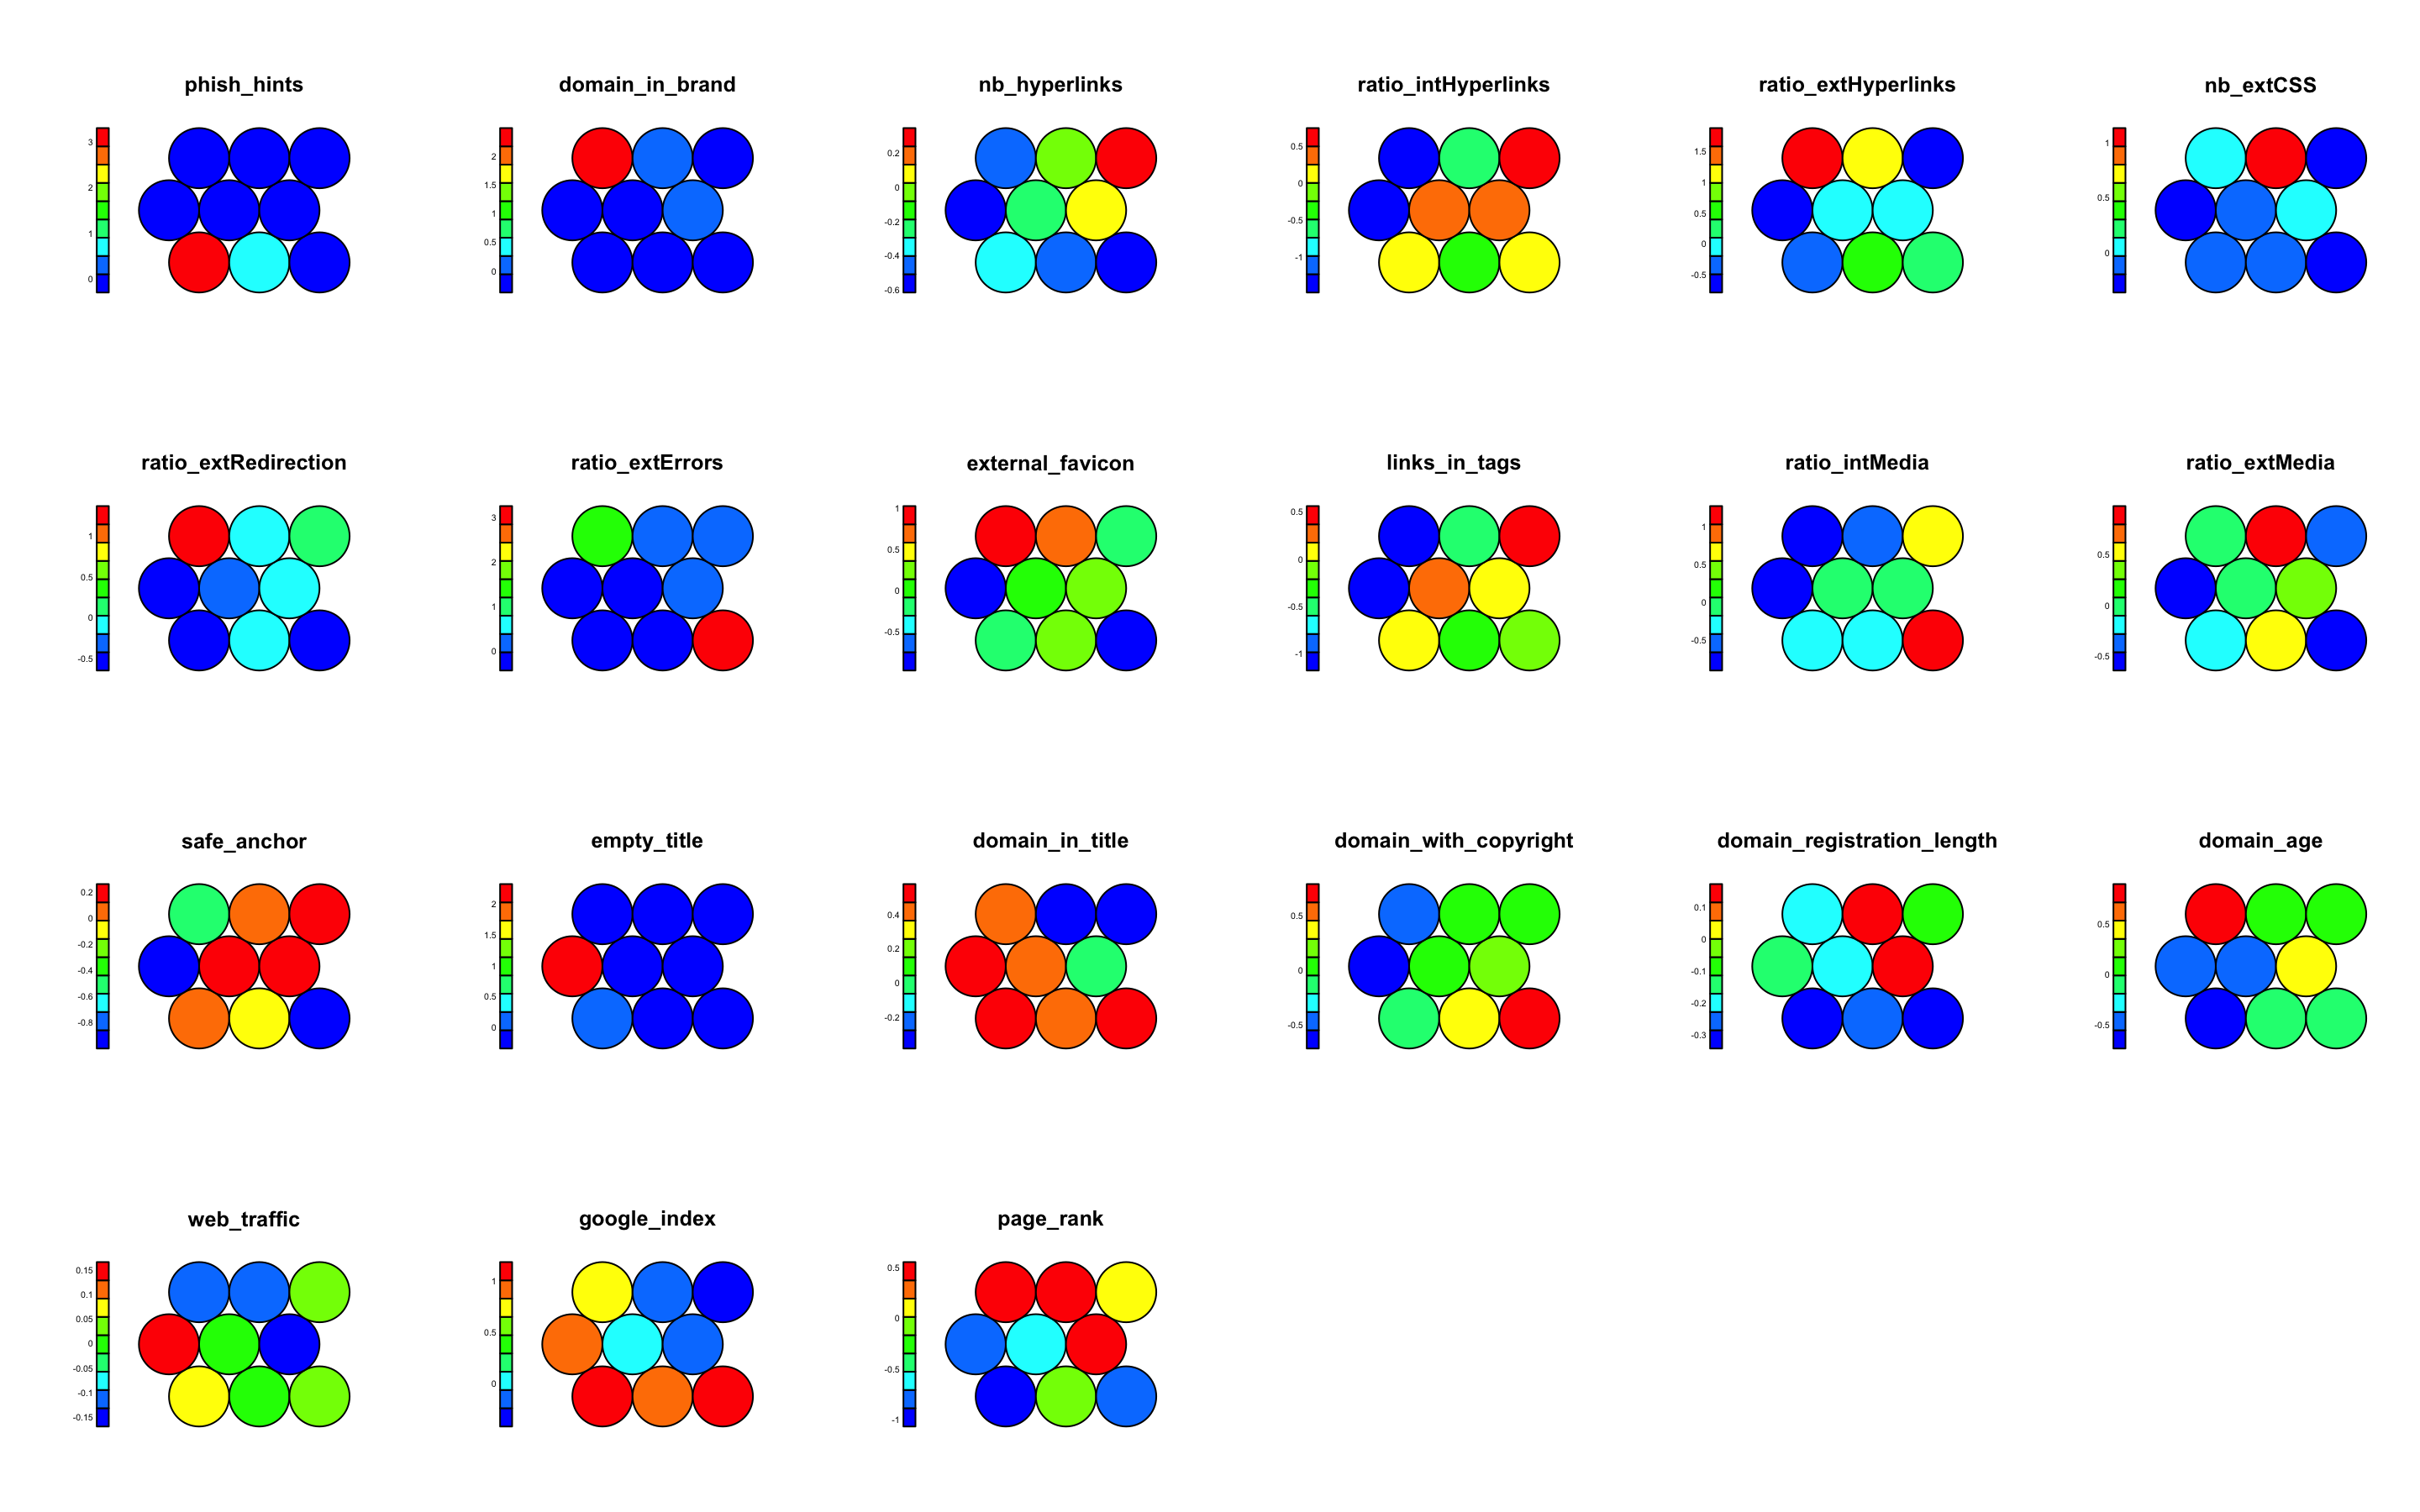
\includegraphics[width=1\textwidth]{maps2.png}
        \caption{Data related to each neuron according to the variable}
        \label{fig:maps.png}
      \end{figure}

      \begin{figure}[H]
        \centering
        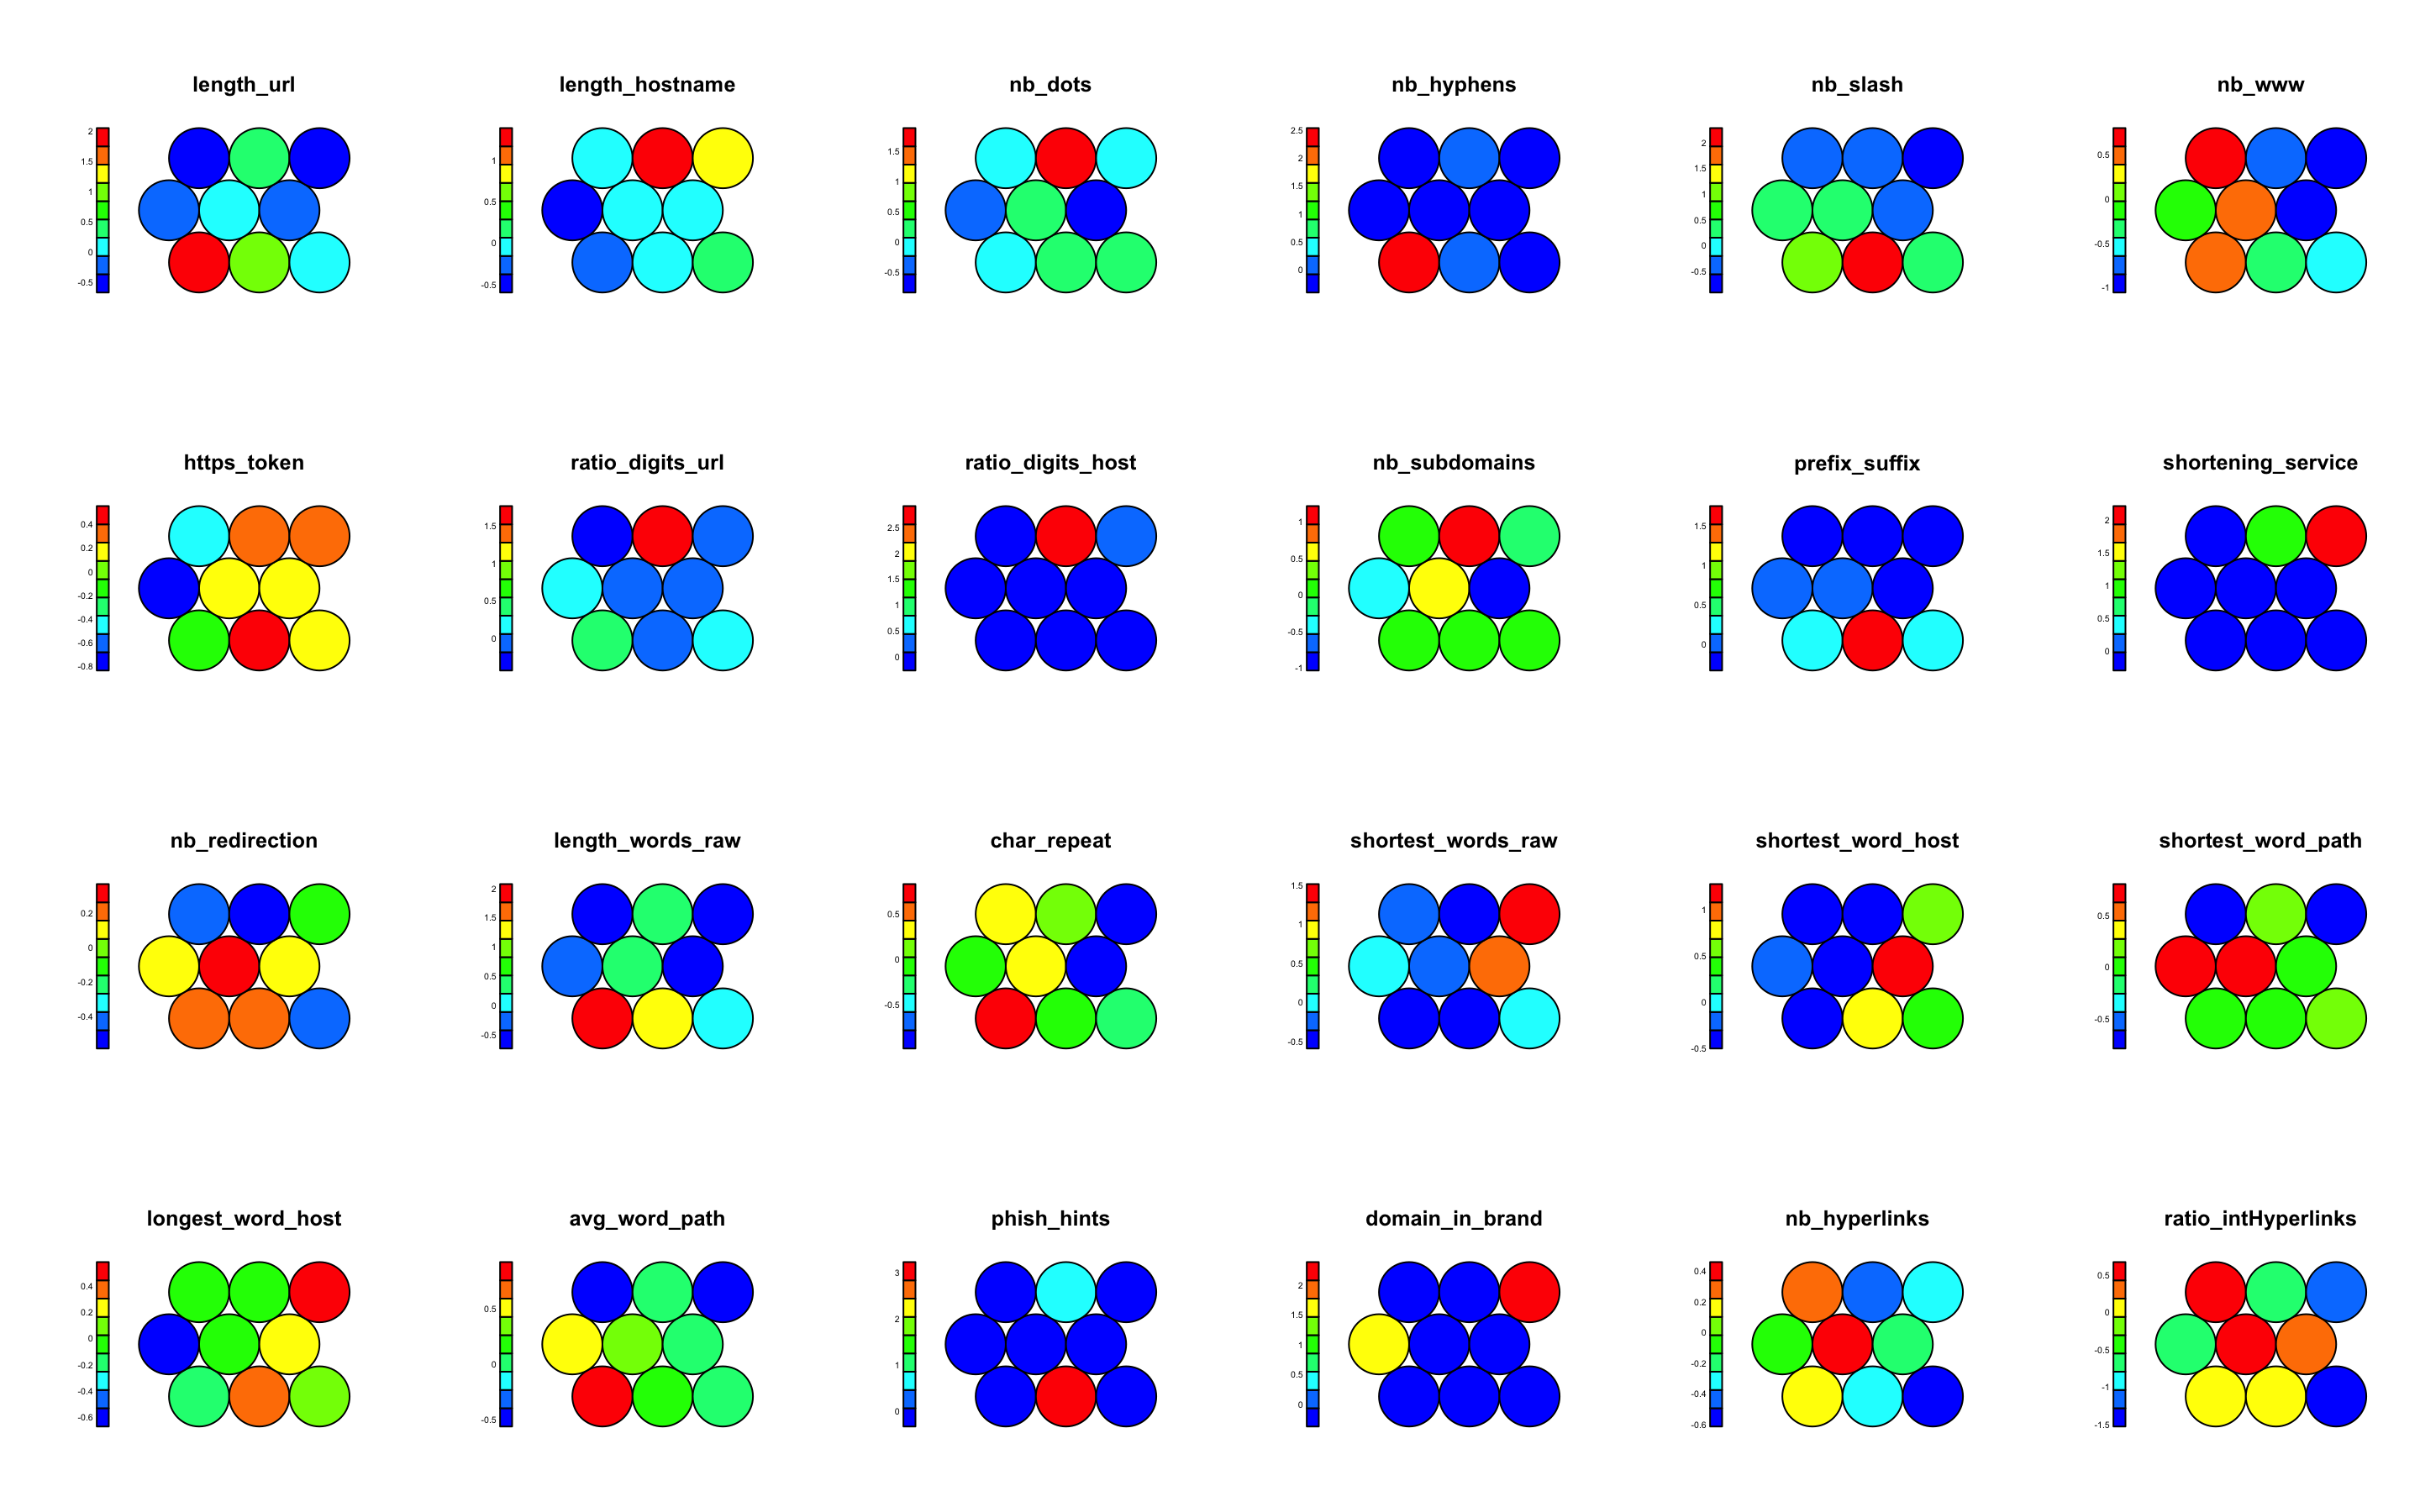
\includegraphics[width=1\textwidth]{maps1_nr.png}
        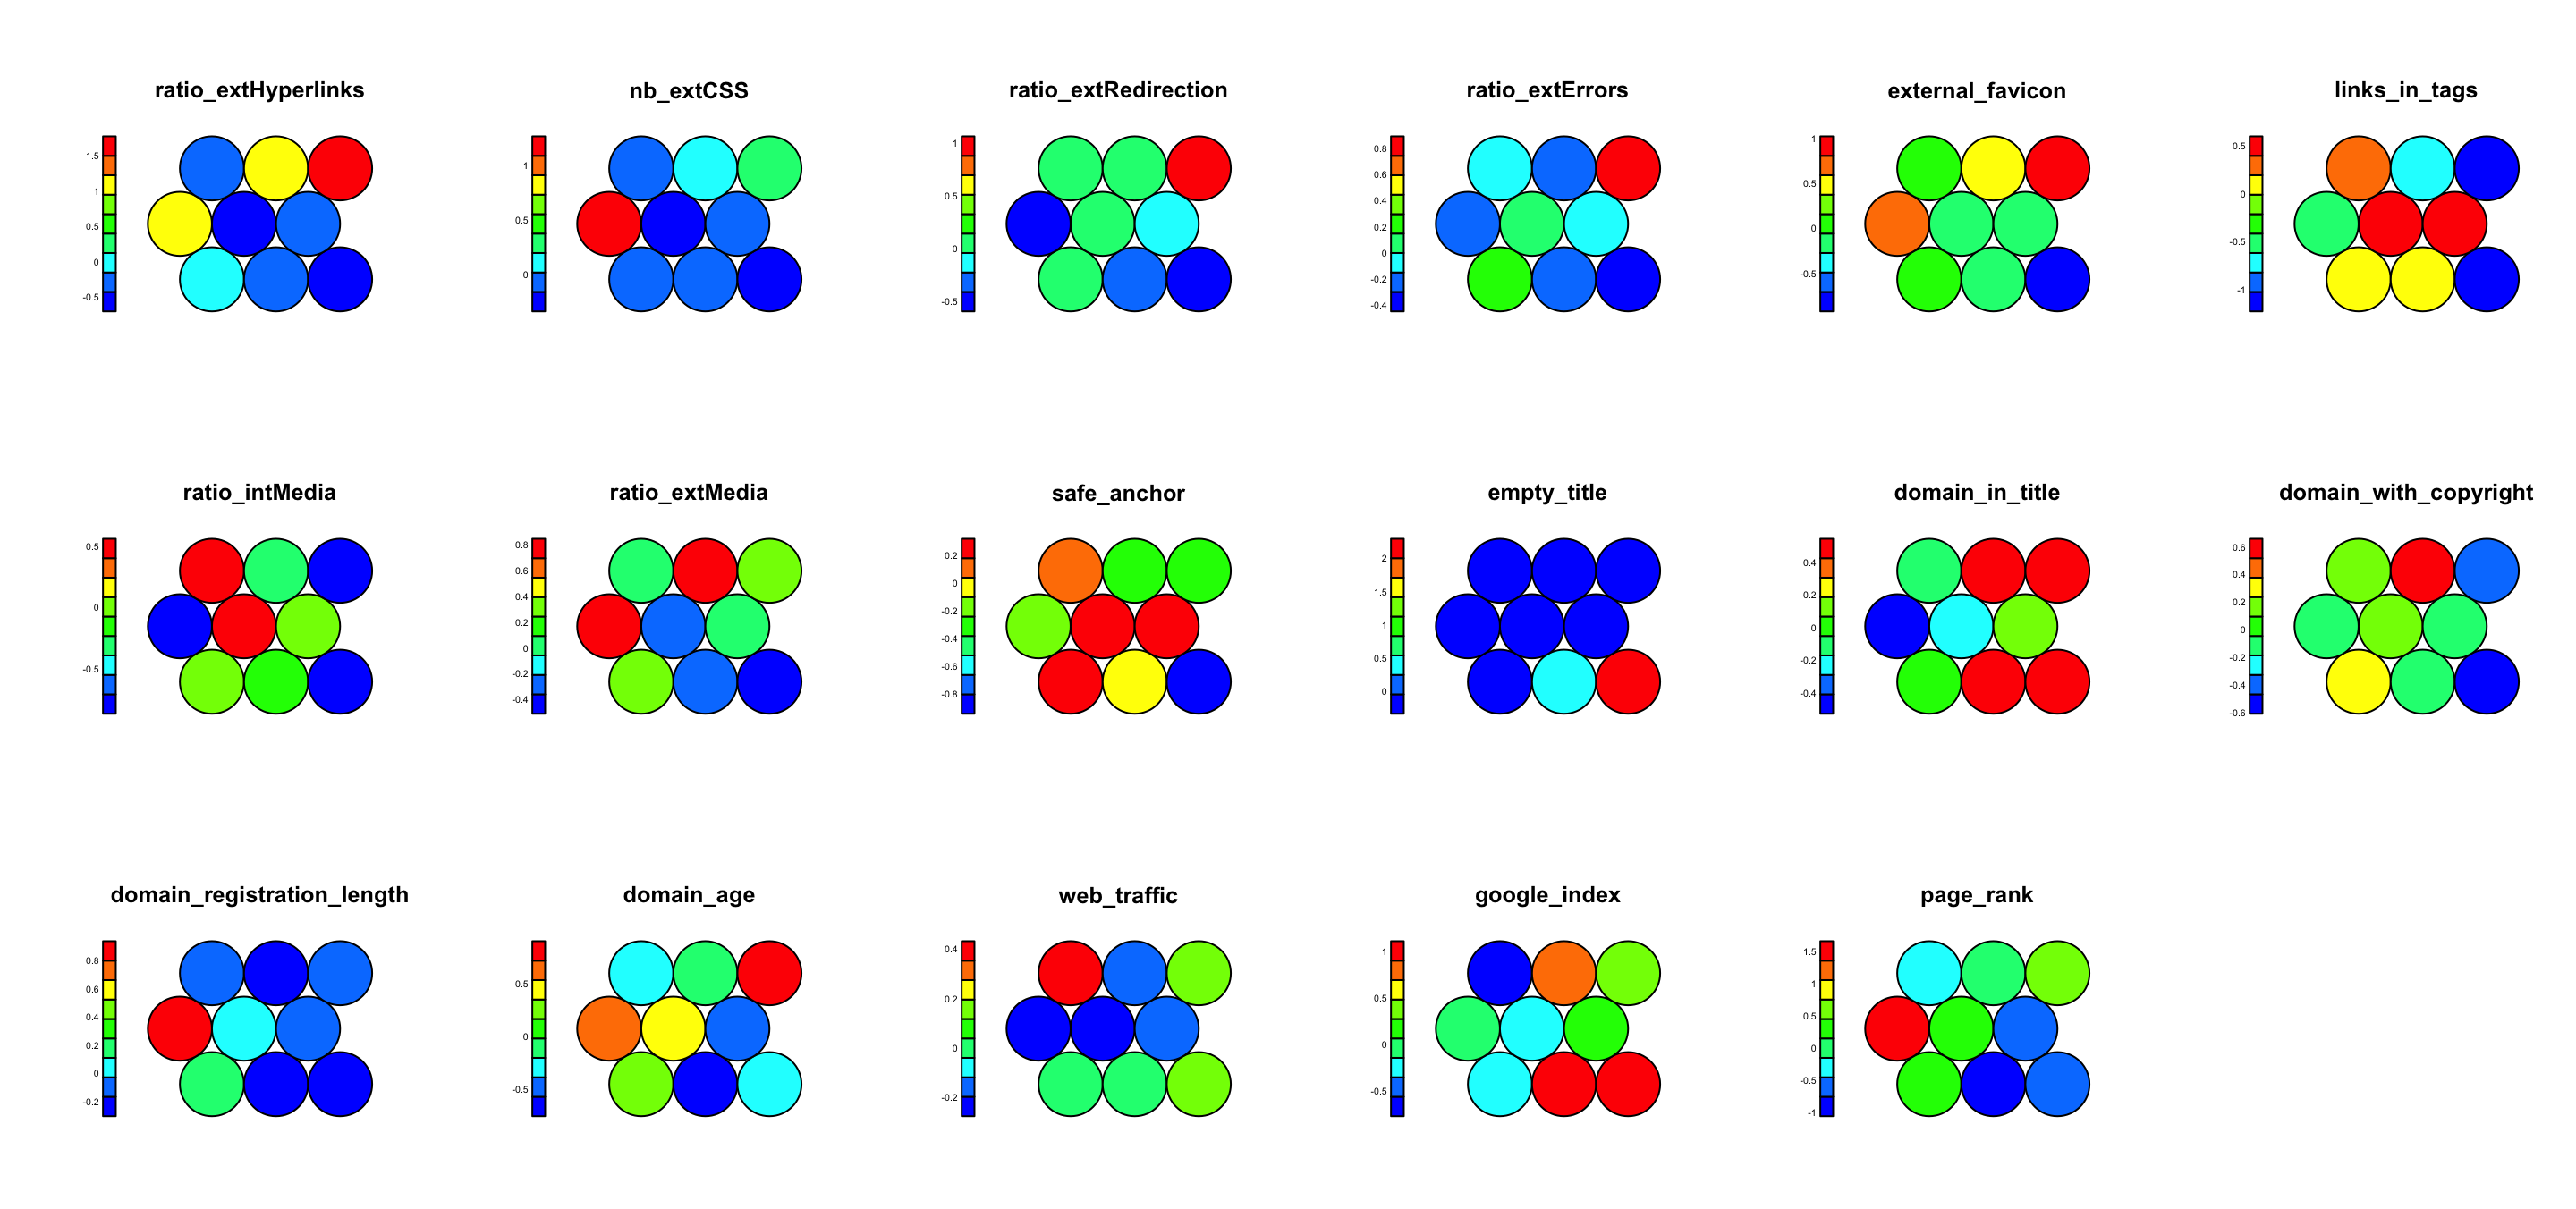
\includegraphics[width=1\textwidth]{maps2_nr.png}
        \caption{Data related to each neuron according to the variable (without redundancies)}
        \label{fig:maps_nr.png}
      \end{figure}

      Once the model is built, a hierarchical clustering is performed over the discovered patterns in the neurons. Indicating $2$ clusters, the \figref{cluster_som.png} is obtained.

      This model is hard to analyze since it does not provide enough information about the data. The formed groups do not have a reasonable meaning, as it happened in hierarchical clustering and \kmeans.

      \figcaption{cluster_som.png}{Clustering of the patterns discovered on each neuron}{1}

    \subsection{Supervised model}

      In this section the same Kohonen algorithm and parameters are used, but this time the algorithms knows the class correspondance of the observations to build the model.

      A common feature of self-organizing maps is that, as it name tells, the data associated to each neuron tend to be sorted according to their similarities. This fact can be seen in \figref{classes_som.png}, where all type $1$ classes (legitimate URL) are separated from type $2$ classes (phishing URL).

      \figcaption{classes_som.png}{Classes of the observations relative to each neuron}{1}

      Then, the model can be tested using confusion matrices for the training and testing sets, as shown below. The resulting precision is \SI{88.79}{\percent} for training and \SI{87.44}{\percent} for testing.

      \begin{minted}[bgcolor=bgcolor]{text}
Train:
             Reference
Prediction   legitimate   phishing
legitimate         2413        138
phishing            320       1213

Test:
             Reference
Prediction   legitimate   phishing
legitimate          783         45
phishing            126        407
      \end{minted}

      These results are acceptable, although a greater precision could be achieved with other algorithm or adding more complexity to the map.

  \section{KNN}

    Another classification model can be done with KNN ($K$-Nearest-Neighbours). It is an algorithm that uses the training set directly to predict the class of the elements that are introduced to the model as input.

    The training set contains \SI{75}{\percent} of the dataset, and the rest is included in the testing set. The optimum value of $K$ is $5$, which means that the entering observation to the model is being compared to the $5$ nearest elements of the training set (its neighbours) and the assigned class will be the predominant one among the neighbours. For this model, the Euclidean distance is used.

    When introducing the testing set, the following confusion matrix is obtained, with a \SI{94.35}{\percent} precision:

    \begin{minted}[bgcolor=bgcolor]{text}
             Reference
Prediction   legitimate   phishing
legitimate          800         49
phishing             28        485
    \end{minted}

    As it is shown, this classification method is pretty good, due to a high precision is achieved and using an algorithm that does not need a training stage.

  \section{Decision trees}

    Following with the classification of the URL, it is intended to analyze several model based on decision trees.

    Firstly, some CART and C4.5 trees are constructed using \texttt{rpart} and \texttt{C50} packets, respectively. And secondly, a model is built with \texttt{randomForest}.

    \subsection{CART}

      Setting a proportion of \SI{75}{\percent} of the dataset for the training set, a CART decision tree is made with default parameters. The resulting tree is the one in \figref{cart.png}.

      \figcaption{cart.png}{CART decision tree}{1}

      Next, the confusion matrices are shown for the training and testing sets:

      \begin{minted}[bgcolor=bgcolor]{text}
Train:
             Reference
Prediction   legitimate   phishing
legitimate         2422        167
phishing            129       1366

Test:
             Reference
Prediction   legitimate   phishing
legitimate          794         53
phishing             34        480
      \end{minted}

      Although the got precisions are high (\SI{92.75}{\percent} for training and \SI{93.61}{\percent} for testing), it is reasonable to think that the tree has unnecessary complexity. The following \figref{cart_cp.png} shows the error the tree obtains depending on the number of nodes (splits) and the cost-complexity parameter:

      \figcaption{cart_cp.png}{Error evolution depending on the number of nodes and the cost-complexity}{1}

      If a pruning process is performed, with a cost-complexity parameter of $0.014$, the resulting tree is simpler:

      \figcaption{cart_pruned.png}{Pruned CART decision tree}{1}

      This time, the precision decreases to \SI{91.41}{\percent} for training and \SI{91.70}{\percent} for testing.

      \begin{minted}[bgcolor=bgcolor]{text}
Train:
             Reference
Prediction   legitimate   phishing
  legitimate       2444      244
  phishing          107     1289

Test:
             Reference
Prediction   legitimate   phishing
legitimate          798         83
phishing             30        450
      \end{minted}

      Looking at the tree in \figref{cart_pruned.png}, one can notice that \texttt{google\_index} is an important variable, due to the fact that if an URL is listed in Google (\texttt{google\_index=0}), then the tree will classify it directly to a legitimate website.

    \subsection{C4.5}

      In this section, a C4.5 decision tree is implemented to make a comparison with the previous CART decision tree.

      Using \texttt{C50} packet of R with the default parametes (confidence factor of $0.25$), a quite complex tree is obtained (with a total of $47$ leave nodes). It follows that the model is overlearning, just taking a look at the resulting confusion matrices.

      \begin{minted}[bgcolor=bgcolor]{text}
Train:
             Reference
Prediction   legitimate   phishing
legitimate         2519         39
phishing             32       1494

Test:
             Reference
Prediction   legitimate   phishing
legitimate          805         26
phishing             23        507
      \end{minted}

      Although these precisions are \SI{98.26}{\percent} and \SI{96.4}{\percent} for training and testing, it is preferred to use the CART pruned tree, because it is simpler and does not contain specific cases as the C4.5 model.

    \subsection{Random forest}

    For this model the fact that the algorithm has a bootstrap process befor generating each tree is taken into advantage, so that it is not necessary to split the dataset in a training set and a testing set.

      As an initial model, the bagging method is performed using the \texttt{randomForest} function with $45$ predictors and $500$ trees. This model achieves an out-of-bag (OOB) error of \SI{1.82}{\percent} (\SI{98.18}{\percent} precision).

      \begin{minted}[bgcolor=bgcolor]{text}
             Reference
Prediction   legitimate   phishing
legitimate         3335         44
phishing             55       2011
      \end{minted}

      It can be seen that this model is so good. However, it can be tweaked with the random forest method, that is, avoiding the use of all the available predictors ($45$). The OOB error evolution according to the number of predictors is shown in \figref{mtry.png}, being $3$ the optimum number of predictors.

      \figcaption{mtry.png}{OOB error evolution depending on the number of predictors}{1}

      Having chosen this parameter, the node size of the tree is adjusted. In the following \figref{nodesize.png} it is presented a graph showing the evolution of the OOB error according to the node size. In this case, the optimum value is $1$.

      \figcaption{nodesize.png}{OOB error evolution depending on the node size}{1}

      \figcaption{trees.png}{OOB error evolution depending on the number of trees}{1}

      \newpage

      The last step is to adjust the number of trees, choosing the number that obtains the least OOB error. In \figref{trees.png} it can be seen how the error changes depending on the number of trees. The minimum error is obtained with $141$ trees.

      Once these parameters are configured, the random forest model is built and it obtains an OOB error of \SI{1.6}{\percent} (\SI{98.4}{\percent} precision), with the following confusion matrix:

      \begin{minted}[bgcolor=bgcolor]{text}
             Reference
Prediction   legitimate   phishing
legitimate         3340         39
phishing             48       2018
      \end{minted}

      This model has a great performance. Overlearning is not critical because the model is based on simple decision trees.

      In addition, the importance of the variables can be computed, as it is represented in \figref{importance.png}. It was deduced that \texttt{google\_index}, \texttt{page\_rank} and \texttt{nb\_hyperlinks} are important (precisely the ones that are present in the CART pruned tree of \figref{cart_pruned.png}).

      \figcaption{importance.png}{Importance of the variables in the random forest model}{1}

  \newpage

  \section{Multi-layer perceptron}

    The last analysis to be performed is the multi-layer perceptron, based on neural networks. The algorithm is in the \texttt{neuralnet} packet of R, which needs the number of layers of the network, the number of neurons per layer and the type of output function (linear or sigmoidal) to be specified.

    After making several experiments with these parameters, it is seen that the best neural network is obtained with two layers containing $6$ and $3$ neurons (hidden layer and output layer, respectively). The output activation function is linear. A representation of the built network can be seen in \figref{nn.png}:

    \figcaption{nn.png}{Implemented neural network}{1}

    Although the output variable \texttt{status} is categorical, the multi-layer perceptron was implemented to return a continuous variable as a result. Initially, the model was built with an output categorical variable, but the algorithm was not able to converge. Consequently, the returning value of the neural network is rounded to the nearest integer number.

    The following \figref{nn_test.png} shows the output of the multi-layer perceptron, before rounding, for the testing set. It can be observed that the vast majority of predictions are very close to values $1$ and $2$ (corresponding to legitimate URL and phishing URL, respectively), so that the discretization does not affect the final result drastically.

    \figcaption{nn_test.png}{Representation of real data and predictions}{1}

    To analyze the performance of this model, the prediction of the data in the training set obtained a \SI{99.51}{\percent} precision. On the other hand, the prediction of the testing set resulted in a \SI{97.5}{\percent} precision. Both confusion matrices are shown below:

    \begin{minted}[bgcolor=bgcolor]{text}
Train:
             Reference
Prediction   legitimate   phishing
legitimate         2542         11
phishing              9       1521

Test:
             Reference
Prediction   legitimate   phishing
legitimate          810         16
phishing             18        518
      \end{minted}

      With these model the resulting precision is really high, proving that the multi-layer perceptron is extremely powerful when classifying observations in a dataset.

  \newpage
  \section*{Conclusions}
    \addcontentsline{toc}{section}{Conclusions}

    Having performed all of the previous \ML\ models, it can be concluded that clustering algorithms are not appropriate for the analysis of the dataset, since they do not seem to group obervations according to the class of the URL.

    On the other hand, classification algorithms are adequate, because the objective is precisely to classify URL by their type (legitimate or phishing). The resulting models ordered by precision in testing stage are shown below:

    \begin{itemize}
      \item Random forest
      \item Multi-layer perceptron
      \item C4.5 decision tree
      \item KNN
      \item Pruned CART decision tree
      \item Supervised Kohonen maps
    \end{itemize}

    If one of these models were used to analyze URL from the Internet and detect potential phishing attacks, the best methods would be random forests and multi-layer perceptron. These models get a extremely high precision.

    It is also considerable to implement KNN, as it is an algorithm that does not need a training process and compares the input data with the ones of the dataset to determine the resulting class. Plus, it also achieves a high precision.

    It is worth mentioning that there are not many false negatives in the obtained confusion matrices (that is, the model classifies a phishing URL as a legitimate one), which is one of the aspects that is desired to minimize.

    Another valid conclusion is that the initial pruning of the dataset has not been critical to build the models, showing that it was a right approach.

  \newpage

  \section*{Annex: Script to characterize an URL}
    \addcontentsline{toc}{section}{Annex: Script to characterize an URL}

    In this section, the usage of the Python script to characterize a list of URL is explained. The output of the script is ready to perform the predictions of the built models with R.

    It is intended that the program is implemented in command line interface, as shown below:

    \begin{minted}[bgcolor=bgcolor]{bash}
$ cd scripts
$ pip install -r requirements.txt
$ python url_features.py -f url.txt -o output.csv
Results written in output.csv
Time: 33.716389179229736 seconds
    \end{minted}

    Inside the \texttt{url.txt} file, indicated by the \texttt{-f} flag, the URL must be listed as shown in the following example:

    \begin{minted}[bgcolor=bgcolor]{text}
https://www.google.com/
https://www.youtube.com/
https://github.com/
    \end{minted}

    It is worth mentioning that the input URL must be accessible. It is probable that a phishing URL is only accesible during a limited period of time. Consequently, it is probable that some URL of the dataset that match phishing will not be characterized because they are not available on the Internet.

    The obtained result for the accessible URL is written into a file whose name is specified with \texttt{-o} flag, CSV format (by default, the output is written to \texttt{output.csv}).

    Once having the CSV file, the type of the URL could be predicted using the built models with R and the following functions:

    \begin{itemize}
      \item \texttt{predict\_using\_randomforest(file)}
      \item \texttt{predict\_using\_mlp(file)}
      \item \texttt{predict\_using\_C50(file)}
      \item \texttt{predict\_using\_knn(file)}
      \item \texttt{predict\_using\_rpart(file)}
      \item \texttt{predict\_using\_som(file)}
    \end{itemize}

    For example, the random forest model could be executed and use the corresponding prediction function from the RStudio console:

    \newpage

    \begin{minted}[bgcolor=bgcolor]{r}
> predict_using_randomforest(file = 'scripts/output.csv')
                         url       status
1    https://www.google.com/   legitimate
2   https://www.youtube.com/   legitimate
3        https://github.com/   legitimate
    \end{minted}

    Finally, the predicted results by the model are simply obtained and clearly shown.

\end{document}
